%%%%%%%%%%%%%%%%%%%%%%%%%%%%%%%%%%%%%%%%%%%%%%%%%%%%%%%%%%%%%%%%%%%%%%%%%%%%%%%%%%%%%%%%%%%%%
%%									Chapitre 1											%
%%%%%%%%%%%%%%%%%%%%%%%%%%%%%%%%%%%%%%%%%%%%%%%%%%%%%%%%%%%%%%%%%%%%%%%%%%%%%%%%%%%%%%%%%%%%%
\chapter{Exploration de l'entreprise}
	\minitoc

%%%%%%%%%%%%%%%%%%%%%%%%%%%%%%%%%%%%%%%%%%%%%%%%%%%%%%%%%%%%%%%%%%%%%%%%%%%%%%%%%%%%%%%%%%%%%




% Début du chapitre

\section{Le rôle du laboratoire Soleil}

	\subsection{Secteur d'activit\'e}
				Le laboratoire SOLEIL a un secteur d'activités tertiaires, les personnes y travaillant font des recherches. 
				Des personnes venant du monde entier viennent faire des recherches au synchrotron SOLEIL parce qu'il existe seulement deux accélérateur de particules en France. Le premier se situe à Paris et se nomme le synchrotron SOLEIL, le second se trouve à Grenoble qui lui est un synchrotron européen donc une partie appartient aux francais et le reste à d'autre pays européen.
	\subsection{Moyens}
		\subsubsection{Personnels}
				En décembre 2015, 432 personnes travaillent au laboratoire SOLEIL.L'âge moyen des salariés est de 44 ans. 5 personnes souffrant d'un handicap travaillent à SOLEIL. 8 ans est l'âge moyen de l'ancieneté des employés.
				75\% , c'est à dire 267, des salariés SOLEIL sont des hommes; 150 sont cadres et 117 sont non cadres.
				25\% , donc 80 des personnes embauchées à SOLEIL sont des femmes\; 42 sont cadres et 38 sont non cadres.


		\subsubsection{Équipements}
			
			\paragraph{L'accélérateur d'électrons}
				La plus grande machine du synchrotron SOLEIL\: l'accélérateur d'éléctrons.
				L'accélérateur d'éléctrons permet d'observer de très petites particules grâce à la lumière émise par les éléctrons.
				Un canon est activité et va envoyer une grande énergie éléctrique qui va séparer les éléctrons du noyau de l'atome. Les éléctrons vont sortir du canon avec une vitesse très rapide. Ensuite les éléctrons vont passer par des aimants qui les accélérer encore plus puis ils vont dans le booster dans lequel ils vont gagner de l'énergie. Ensuite les éléctrons sont envoyer dans l'anneau de stockage, où ils tournent pendant pusieurs heures et où ils avancent à une vitese proche de celle de la lumière. Dans l'anneau de stockage il y a des virages où les éléctrons doivent tourner et subissent des accélérations. Quand ils accélèrent ils libèrent des photons, ou lumière. Ses photons vont être utilisés dans les lignes de lumières, où les scientifiques vont expérimenter la réaction de la lumière sur des objets ou inversement. Les lignes de lumières sont composés de trois cabanes; la cabane optique, la cabane d'expériences et la cabane de vie. Dans la cabane optique on trouve des miroirs déviant la lumière. La cabane d'expériences est l'endroit où on pose l'échantillom a observer et la cabane de vie est l'endroit où on observe l'échantillon et où les scientifiques règlent la caméra. 
			
			\paragraph{Les Aimants}
				Pour faire tourner les éléctrons et les garder ensemble, des aimants sont utilisés. Plusieurs aimants sont utilisés à SOLEIL. Il y a le dipôle; qui comporte deux aimants et qui fait dévier les éléctrons du côté choisi.Les quadrupôles servent à resserer les éléctrons entre eux parce que quand les éléctrons tournent, ils ont plus de places et donc essaient de s'él;oigner car deux charges négatives se rejettent. Les aimants nommés sextupôles font la même chose que les quadrupôles mais plus précisement.Pour alimenter les aimants en éléctricité, on utilise des alimentations. Il existe 32 dipôles, 160 quadripôles et 120 sextupôles au synchrotron SOLEIL. Les dipôles et les quadripôles sont dans l'anneau de stockage et le booster au contraire des sextupôles qui ne se trouvent que dans l'anneau de stockage. Les dipôles et les quadrupôles sont plus grand que dans l'anneau de stockage.
			
			\paragraph{Autres équipements}
				Le synchrotron SOLEIL possède trois imprimante 3D avec lesquels ils fabriquent de petites pièces. On peut voir beaucoup d'ordinateur, dans chaque salle on voit un ou plusieurs ordinateurs; dans la salle de commande, les salles de vie dans les lignes de lumière, les bureaux d'ingénieurs, de dessinateur projecteur, des mécaniciens, des scientifiques... Les aligneurs possèdent des niveaux qui permettent de positionner tous les équipements pour les lignes des lumières. Des pompes sont utilisés par les videurs pour faire le vide dans les tubes de l'accélérateur d'éléctrons.



\section{Exemple minimal}
	\subsection{Glossaire et citations}
		On va raconter n'importe quoi à propos des \gls{asb}, juste pour illustrer à quoi ressemblent les différents glossaires. On pourrait tout aussi bien converser sur la pertinence de l'utilisation des \gls{csl} pour caractériser les \glspl{macle} du \gls{rutile}. Et pour craner un peu, je vais citer le merveilleux travail de \citet{depriester2014thermomechanical}. Maintenant que les \gls{asb} et \gls{csl} ont été définies, plus besoin de détailler leurs significations.
		
	\subsection{Tableaux et figures}
	On va ici placer des éléments graphiques (voir tableau~\ref{tab:exemple} et figure~\ref{fig:exemple}), juste pour avoir des entrées dans les listes des figures et des tableaux. On remarquera l'utilisation des sous-figures~\ref{sub:Antibes} et~\ref{sub:SaintJeannet}.
	
	\begin{tableth}
		\caption[Légende courte pour l'exemple de tableau]{Un tableau avec une légende tellement longue que ce serait hideux dans la liste des tableaux}
			\label{tab:exemple}
		\begin{tabular}{c|c}
			Coucou	& Au revoir\\
			\hline
			maman	& papa
		\end{tabular}
	\end{tableth}

	\begin{figureth}
		\begin{subfigureth}{0.4\textwidth}
			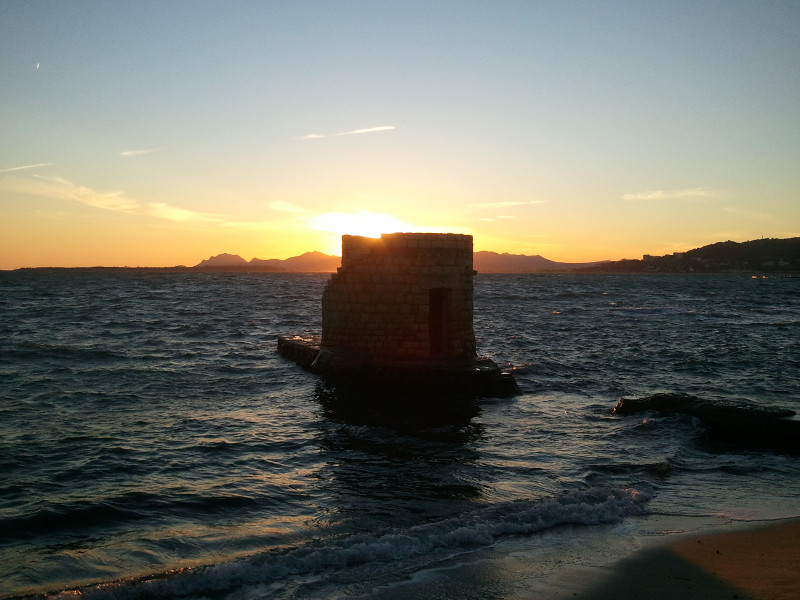
\includegraphics[width=\linewidth]{Antibes}
			\caption{Photo du Cap d'Antibes}
				\label{sub:Antibes}
		\end{subfigureth}
		\begin{subfigureth}{0.4\textwidth}
			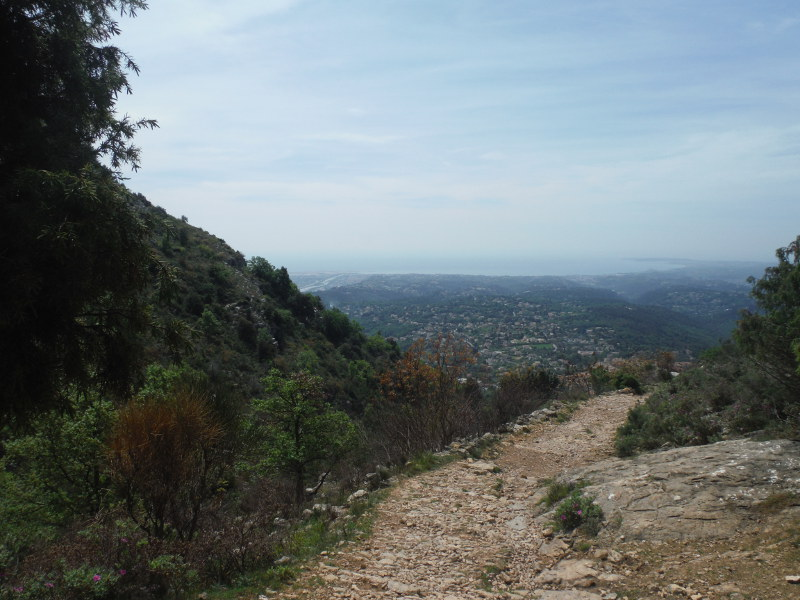
\includegraphics[width=\linewidth]{SaintJeannet}
			\caption{Saint Jeannet, depuis son Baou}
				\label{sub:SaintJeannet}
		\end{subfigureth}
		\caption[Légende courte pour la figure]{Exemple d'utilisation des sous-figures. J'utilise ici volontairement une légende longue.}		
			\label{fig:exemple}
	\end{figureth}
	
	\subsection{Symboles mathématiques}
	Rien de spécial à propos des math, hormis l'illustration des symboles listés en fin de document, tels \gls{alpha} ou \gls{gamma}, qui peuvent être utilisés indifféremment en mode \emph{in-line} ou dans des équations\footnote{Le lecteur notera que \texttt{hyperref} ajoute un lien cliquable sur chaque entrée des différents glossaires.} :
	\begin{equation}
		\gls{alpha}=\nicefrac{\gls{gamma}}{2}
		\label{eq:alphagamma}
	\end{equation}
Les entrées des glossaires peuvent même être appelés dans des figures (PDF avec surcouche \LaTeX, ou Ti\textit{k}Z).
	

\section{Deuxième paragraphe}
\blindtext

\bibliographystyle{francaissc}
\bibliography{Chapitre1/Biblio}